
Section~\ref{sec:background} described four families that all compress $t$
ephemeral secrets into one seed tree and then decide, per node, which seeds may
be released. We now isolate that mechanism, define the signature scheme built
on top of it, and state the invariant that the decision must satisfy.

\subsection{The seed-tree mechanism}

\begin{definition}[\GZKST]
\label{def:gzkst}
A \emph{Generic ZK Seed Tree} (\GZKST) is a tuple
$\Pi = (\Setup,\, \Expand,\, \Chal,\, \Decide,\, \Publish,\, \Recon)$
parametrised by a security parameter $\lam$, a number $t \in \mathbb{N}$ of
parallel repetitions, and a pseudorandom generator
$\PRG : \{0,1\}^{\lam} \to \{0,1\}^{2\lam}$. The six algorithms are:
\begin{multicols}{2}
\begin{enumerate}[leftmargin=*,itemsep=2pt]
  \item $\Setup(1^{\lambda}) \to (\seed_r,\salt)$: samples a master seed
        $\seed_r \getsr \{0,1\}^{\lambda}$ and a public salt.

  \item $\Expand(\seed_r,\salt) \to (\calT,(\eseed_0,\ldots,\eseed_{t-1}))$:
        builds a binary tree $\calT$ by top-down \PRG-expansion from
        $\seed_r$, leaf $i$ holding $\eseed_i$. The topology may be complete
        or incomplete.

  \item $\Chal(\cmt_0,\ldots,\cmt_{t-1},\msg) \to
        \mathbf{c} = (c_0,\ldots,c_{t-1})$: derives a fixed-weight
        Fiat--Shamir challenge from the round commitments and the message.

  \item $\Decide(\mathbf{c}) \to (\calH,\calR)$: partitions
        $\{0,\ldots,t-1\}$ into the hidden set $\calH = \{i : c_i \neq 0\}$,
        $|\calH| = w$, and the revealed set $\calR = \{i : c_i = 0\}$.

  \item $\Publish(\calT,\calH) \to \tpath$: returns a set of nodes from which
        every $\eseed_i$ with $i \in \calR$ is reconstructible and no
        $\eseed_i$ with $i \in \calH$ is derivable.

  \item $\Recon(\tpath,\mathbf{c},\salt) \to \{\eseed_i : i \in \calR\}$:
        verifier-side reconstruction of the revealed leaf seeds.
\end{enumerate}
\end{multicols}
\end{definition}

Definition~\ref{def:gzkst} describes only the seed machinery; it says nothing
about secrets or messages. To speak about key recovery we must say how a
signature scheme is built on top of it, which is the content of the next
definition.

\subsection{The derived signature scheme}
\label{sec:derived}

\begin{definition}[Round functions]
\label{def:round}
A \emph{round system} for a \GZKST\ $\Pi$ over a secret type $\calS$ (the type
of the long-term secret: monomial permutations for LESS, matrix pairs for
MEDS, an R-SDP solution for CROSS, a witness for MPCitH) is a triple
$(\Commit, \Resp, \ChkRnd)$ of efficient algorithms:
\begin{itemize}[leftmargin=*]
  \item $\Commit(\eseed_i, \salt, i) \to \cmt_i$: derives the round-$i$
        ephemeral secret from the leaf seed and commits to it. It does not
        take $\sk$.
  \item $\Resp(\eseed_i, c_i, \sk) \to \resp_i$: for a hidden round, combines
        the ephemeral secret with the component of $\sk \in \calS$ selected by
        $c_i$.
  \item $\ChkRnd(\resp_i, c_i, \pk, i) \to \cmt_i$ or $\perp$: recomputes the
        round-$i$ commitment from the response alone, without $\eseed_i$.
\end{itemize}
\end{definition}

\begin{definition}[Derived signature scheme]
\label{def:sigma}
Given $\Pi$ and a round system as above, the \emph{derived signature scheme}
$\Sig[\Pi]$ is the pair $(\Sign, \Verify)$ of Algorithm~\ref{alg:generic}.
\end{definition}

\begin{figure}[htbp]
\centering
\begin{minipage}[t]{0.48\textwidth}
\begin{algorithm}[H]
\footnotesize
\setlength{\algomargin}{0.7em}
\caption{$\Sig[\Pi].\Sign$}
\label{alg:generic}
\KwIn{Secret key $\sk$, message $\msg$}
\KwOut{Signature $\sig$}
$(\seed_r,\salt) \leftarrow \Setup(1^{\lam})$\;
$(\calT,(\eseed_i)_i) \leftarrow \Expand(\seed_r,\salt)$\;
\lFor{$i = 0$ \KwTo $t-1$}{$\cmt_i \leftarrow \Commit(\eseed_i,\salt,i)$}
$\mathbf{c} \leftarrow \Chal(\cmt_0,\ldots,\cmt_{t-1},\msg)$\;
$(\calH,\calR) \leftarrow \Decide(\mathbf{c})$\;
\lFor{$i \in \calH$}{$\resp_i \leftarrow \Resp(\eseed_i,c_i,\sk)$}
$\tpath \leftarrow \Publish(\calT,\calH)$\;
\Return $\sig \leftarrow \bigl(\mathbf{c},(\resp_i)_{i\in\calH},\tpath,\salt\bigr)$
\end{algorithm}
\end{minipage}\hfill
\begin{minipage}[t]{0.48\textwidth}
\begin{algorithm}[H]
\footnotesize
\setlength{\algomargin}{0.7em}
\caption{$\Sig[\Pi].\Verify$}
\label{alg:generic-verify}
\KwIn{Public key $\pk$, message $\msg$, signature $\sig$}
\KwOut{$\mathsf{accept}$ or $\perp$}
Parse $\sig$ as $(\mathbf{c},(\resp_i)_{i\in\calH},\tpath,\salt)$\;
$(\calH,\calR) \leftarrow \Decide(\mathbf{c})$\;
$\{\eseed_i\}_{i \in \calR} \leftarrow \Recon(\tpath,\mathbf{c},\salt)$\;
\lFor{$i \in \calR$}{$\widehat{\cmt}_i \leftarrow \Commit(\eseed_i,\salt,i)$}
\lFor{$i \in \calH$}{$\widehat{\cmt}_i \leftarrow \ChkRnd(\resp_i,c_i,\pk,i)$}
\lIf{some $\widehat{\cmt}_i = \perp$}{\Return $\perp$}
\lIf{$\Chal(\widehat{\cmt}_0,\ldots,\widehat{\cmt}_{t-1},\msg) = \mathbf{c}$}
   {\Return $\mathsf{accept}$}
\Return $\perp$
\end{algorithm}
\end{minipage}
\end{figure}

\begin{remark}
MEDS instantiates Definition~\ref{def:round} by setting
\[
  \Commit(\sigma_i,\alpha,i) \;=\;
  \Compress\bigl(\SF(\pimap{\tilde{A}_i}{\tilde{B}_i}(G_0))\bigr),
\]
with $\Resp$ given by~\eqref{eq:meds-resp} and $\ChkRnd$ applying
$(\mu_i,\nu_i)$ to $G_{h_i}$. Comparing Algorithm~\ref{alg:generic} with
Algorithm~\ref{alg:sign_meds}, the digest $d$ plays the role of $\mathbf{c}$
and line~14 is $\Publish$.
\end{remark}
% ------------------------------------------------------------
\textbf{The Flag Structure.}
The flag structure $\calF$ produced internally by $\Publish$ is the key
intermediate object.  It is a labelling $\calF : V(\calT) \to \{0,1\}$ where:
\begin{itemize}
  \item $\calF(v) = 0$: node $v$ is \emph{publishable}---either
        directly included in $\tpath$ or derivable from a published ancestor;
  \item $\calF(v) = 1$: node $v$ is \emph{hidden}---it must not appear in $\tpath$ and must not be derivable from published nodes.
\end{itemize}
The flag structure satisfies two invariants:

Throughout we use the convention $\calF(\mathsf{parent}(\mathrm{root})) = 1$,
so that the root itself may belong to $\tpath$.

\begin{invariant}[Correctness]
\label{inv:correctness}
For every $i \in \calR$ there exists a node $v$ on the path from the root to
leaf $\eseed_i$ such that $\calF(v) = 0$ and $\calF(\mathsf{parent}(v)) = 1$.
\end{invariant}

\begin{invariant}[ZK hiding]
\label{inv:hiding}
For every $i \in \calH$, no ancestor of leaf $\eseed_i$ satisfies $\calF(v) = 0$.
\end{invariant}

The ZK property of the signature scheme is contingent on
Invariant~\ref{inv:hiding} holding for \emph{all} $i \in \calH$. A fault that
changes $\calF(v)$ from $1$ to $0$ for any $v$ that is an ancestor of some
$\eseed_i$ with $i \in \calH$ \emph{breaks Invariant~\ref{inv:hiding}} and
may allow an attacker to reconstruct $\eseed_i$. We provide an example of
the GGM tree, together with the concepts of the hidden tree and flag
structure, in Figure~\ref{fig:less-trees}.


\subsection{Mapping the schemes onto the model}
\label{sec:mapping}

\begin{proposition}[MEDS, LESS-v2 and CROSS are \GZKST\ instances]
\label{prop:meds-gzkst}
MEDS instantiates Definition~\ref{def:gzkst} with secret type
$\calS = \{(A_j^{-1},B_j^{-1})\}_{j=1}^{s-1}$ and a \GGM\ tree of height
$\lceil\log_2 t\rceil$, complete when $t$ is a power of two and otherwise
using only its first $t$ leaves. LESS-v2~\cite{LESS-spec} instantiates it with
$\calS = \{\pi_1,\ldots,\pi_{s-1}\}$ and an incomplete tree whose $\Publish$
is the two-phase flag-tree construction of Section~\ref{sec:others};
CROSS~\cite{CROSSspec} with $\calS = \{\mathbf{e}\}$ and a complete tree whose
$\Publish$ follows MEDS. In all three cases
Invariants~\ref{inv:correctness} and~\ref{inv:hiding} hold by construction.
\end{proposition}

\label{prop:less-gzkst}%
Concretely for MEDS: $\Setup$ derives $(\seed_r,\salt)$ from one $\XOF$ call;
$\Expand$ builds the tree by hashing each parent with the salt and node index;
$\Chal$ expands the leaves, hashes the compressed generators with the message
and parses the digest through $\ParseHash_{s,t,w}$ into a weight-$w$
$\mathbf{h}$; $\Decide$ sets $\calH = \{i : h_i \neq 0\}$; $\Publish =
\SeedTreeToPath_t$ applies $\calF(v) = \calF(\ell) \vee \calF(r)$ bottom-up
and serialises the boundary in depth-first order; and $\Recon =
\PathToSeedTree_t$ re-expands it downward, leaving the positions in $\calH$
empty. The proof (Appendix~\ref{app:proof-meds}) is purely graph-theoretic,
depending only on the OR-propagation
characterisation~\eqref{eq:meds-flag-char}, so it is insensitive to tree
shape; this is what carries it to LESS-v2, whose index-tracking arrays keep
$\LabelLeaves$ and $\ComputeSeeds$ on the correct nodes whatever depth the
leaves sit at. CROSS additionally authenticates
$\{\mathsf{cmt}_0[i]\}_{i\in\calH}$ with a Merkle tree, which is orthogonal to
seed hiding and which we do not model.

\begin{remark}
This $\Publish$ follows the MEDS submission~\cite{MEDS_PQC}; the reference
implementation uses a different algorithm, detailed in Section~\ref{sec:app}
and revisited in Remark~\ref{rem:spec-vs-impl}.
\end{remark}

\begin{figure}[tb]
\centering
\begin{minipage}[b]{0.42\linewidth}
\centering
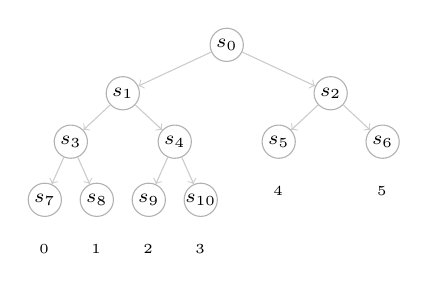
\begin{tikzpicture}[x=0.66cm, y=0.82cm]
  \tikzstyle{neutnode}  = [circle, draw=gray!60, fill=white, text=black, minimum size=12pt, inner sep=0pt, font=\scriptsize]
  \tikzstyle{treeedge} = [gray!40, rounded corners=2pt,->, thin]
  \tikzstyle{leaflbl}  = [font=\tiny, below=1pt]
  \node[neutnode](s0) at (3.5,0){$s_0$};
  \node[neutnode](s1) at (1.5,-.75){$s_1$};
  \node[neutnode](s2) at (5.5,-.75){$s_2$};
  \node[neutnode](s3) at (.5,-1.5){$s_3$};
  \node[neutnode](s4) at (2.5,-1.5){$s_4$};
  \node[neutnode](s5) at (4.5,-1.5){$s_5$};
  \node[neutnode](s6) at (6.5,-1.5){$s_6$};
  \node[neutnode](s7) at (0,-2.4){$s_7$};
  \node[neutnode](s8) at (1,-2.4){$s_8$};
  \node[neutnode](s9) at (2,-2.4){$s_9$};
  \node[neutnode](s10) at (3,-2.4){$s_{10}$};
  \node[leaflbl] at (0,-2.9){$\eseed_0$};
  \node[leaflbl] at (1,-2.9){$\eseed_1$};
  \node[leaflbl] at (2,-2.9){$\eseed_2$};
  \node[leaflbl] at (3,-2.9){$\eseed_3$};
  \node[leaflbl] at (4.5,-2.0){$\eseed_4$};
  \node[leaflbl] at (6.5,-2.0){$\eseed_5$};
  \draw[treeedge](s0)--(s1);\draw[treeedge](s0)--(s2);
  \draw[treeedge](s1)--(s3);\draw[treeedge](s1)--(s4);
  \draw[treeedge](s2)--(s5);\draw[treeedge](s2)--(s6);
  \draw[treeedge](s3)--(s7);\draw[treeedge](s3)--(s8);
  \draw[treeedge](s4)--(s9);\draw[treeedge](s4)--(s10);
  
\end{tikzpicture}
\vspace{2pt}
{\small (a) Expanded reference \GGM\ seed tree.}
\end{minipage}%
\hfill%
\begin{minipage}[b]{0.55\linewidth}
\centering
\begin{tikzpicture}[x=0.66cm, y=0.82cm]
  \tikzstyle{neutnode} = [circle, draw=gray!60, fill=nodehid, text=black, minimum size=12pt, inner sep=0pt, font=\scriptsize]
  \tikzstyle{pubnode}  = [circle, draw=green!50!black, fill=nodepath, minimum size=12pt, inner sep=0pt, font=\scriptsize]
  \tikzstyle{zeronode} = [circle, draw=gray!60, fill=nodepub, minimum size=12pt, inner sep=0pt, font=\scriptsize]
  \tikzstyle{treeedge} = [gray!40, rounded corners=2pt,->, thin]
  \tikzstyle{leaflbl}  = [font=\tiny, below=1pt]
  \node[neutnode](s0) at (3.5,0){$s_0$};
  \node[neutnode](s1) at (1.5,-.75){$s_1$};
  \node[neutnode](s2) at (5.5,-.75){$s_2$};
  \node[neutnode](s3) at (.5,-1.5){$s_3$};
  \node[pubnode] (s4) at (2.5,-1.5){$s_4$};
  \node[neutnode](s5) at (4.5,-1.5){$s_5$};
  \node[pubnode] (s6) at (6.5,-1.5){$s_6$};
  \node[pubnode] (s7) at (0,-2.4){$s_7$};
  \node[neutnode](s8) at (1,-2.4){$s_8$};
  \node[zeronode](s9) at (2,-2.4){$s_9$};
  \node[zeronode](s10) at (3,-2.4){$s_{10}$};
  \node[leaflbl] at (0,-2.9){$\eseed_0$};
  \node[leaflbl] at (1,-2.9){$\eseed_1$};
  \node[leaflbl] at (2,-2.9){$\eseed_2$};
  \node[leaflbl] at (3,-2.9){$\eseed_3$};
  \node[leaflbl] at (4.5,-2.0){$\eseed_4$};
  \node[leaflbl] at (6.5,-2.0){$\eseed_5$};
  \draw[treeedge](s0)--(s1);\draw[treeedge](s0)--(s2);
  \draw[treeedge](s1)--(s3);\draw[treeedge](s1)--(s4);
  \draw[treeedge](s2)--(s5);\draw[treeedge](s2)--(s6);
  \draw[treeedge](s3)--(s7);\draw[treeedge](s3)--(s8);
  \draw[treeedge](s4)--(s9);\draw[treeedge](s4)--(s10);
  
\end{tikzpicture}
\vspace{2pt}
{\small (b) After \Chal, \Decide, \Publish; $\mathbf{b}\!=\!\{0,1,0,0,1,0\}$, $\tpath\!=\!\{s_4,s_6,s_7\}$.}
\end{minipage}
\caption{GGM seed tree ($t=6$): structure~(a) and flag state~(b).
In~(b): pink nodes ($\calF{=}1$, hidden subtree); green nodes ($\calF{=}0$,
fully revealed subtree); blue-bordered nodes ($\calF{=}0$, in $\tpath$).}
\label{fig:less-trees}
\end{figure}


\subsection{The faulted oracle and dual revelation}
\label{sec:oracle}

\begin{definition}[Faulted Signing Oracle]
\label{def:fault-oracle}
Let $\Pi=(\Setup,\Expand,\Chal,\Decide,\allowbreak
\Publish,\allowbreak\Recon)$ be a \GZKST
instance, let $\Sig[\Pi]$ be the derived signature scheme of
Definition~\ref{def:sigma}, and let $(\sk,\pk)$ be a fixed key pair. For a
node $v^*\in V(\calT)$, the oracle $\Oracle^{v^*}(\sk,\pk)$ runs
$\Sig[\Pi].\Sign(\sk,\msg)$ unmodified except that, during
$\Publish(\calT,\calH)$, it forces
$\calF(v^*) \leftarrow 0$
before the normal upward propagation step. The oracle outputs the
resulting (possibly faulted) signature $\sig^*$.
\end{definition}

A fault is \emph{effective} if $v^*$ originally satisfies
$\calF(v^*)=1$ and is an ancestor of some hidden leaf
$\eseed_i$ with $i\in\calH$. In this case, the published path
reveals a node from which $\eseed_i$ is derivable, violating
Invariant~\ref{inv:hiding}. Otherwise, the fault is
\emph{ineffective}.

Definition~\ref{def:fault-oracle} is realised by instruction skips,
stuck-at-zero faults, bit flips and clock
glitches~\cite{ZKFault,FaultToForge2025} alike; the abstraction is indifferent
to which. An honest signature reveals $\resp_i$ for every $i \in \calH$ while
keeping $\eseed_i$ hidden, and an effective fault breaks that separation,
handing the attacker both. We call this \emph{dual revelation}; it is the
primitive underlying every secret-recovery attack in this work.






\subsection{A taxonomy of fault surfaces}
\label{sec:taxonomy}

The value of Definitions~\ref{def:gzkst} and~\ref{def:sigma} is not that they
restate the (obvious) fact that revealing a hidden seed breaks zero knowledge.
It is that they make the fault surface \emph{enumerable}. Every implementation
of $\Sig[\Pi]$ must materialise each of the components in turn, and each
component admits its own class of faults with its own consequence:

\begin{itemize}[leftmargin=*,itemsep=1pt]
  \item $\Setup$: biasing or zeroing $\seed_r$ makes the whole tree, and hence
        every $\eseed_i$, predictable without touching $\Publish$.
  \item $\Expand$: skipping a \PRG\ invocation leaves a child at a known or
        stale value --- the surface exploited against
        FAEST~\cite{JendralD25} and Mirath/RYDE~\cite{BandaBK26}.
  \item $\Chal$: corrupting the digest before parsing changes which rounds are
        hidden; the attack of~\cite{HuangHHYSTY26} skips iterations of the
        digest-preprocessing loop of LESS-v2 and never touches the tree.
  \item $\Decide$: forcing $c_i \leftarrow 0$ moves a round from $\calH$ to
        $\calR$, so its seed is published \emph{legitimately} after $\resp_i$
        has already been emitted.
  \item $\Publish$: corrupting the per-node release decision ---
        \cite{ZKFault,FaultToForge2025} and all three attacks of
        Section~\ref{sec:app}.
  \item $\Recon$: verifier-side, so relevant to acceptance rather than key
        recovery; it matters here because a verify-before-release
        countermeasure runs $\Recon$ on the signer's own device
        (Section~\ref{sec:counter}).
\end{itemize}

Table~\ref{tab:surfaces} places the published attacks on this grid. Two
observations follow. First, five independent attacks developed against four
schemes, with different tree shapes and different secret types, occupy only
three of the six components, which suggests the grid is the right coordinate
system rather than an artefact. Second, the empty cells are predictions: one
of them produced Model~2 of Section~\ref{sec:app}, since asking what
\emph{else} inside $\Publish$ can be faulted besides the flag value points at
the index bookkeeping that walks the tree --- a surface with no analogue in the
LESS flag array, and one no previous work had considered.

\begin{table}[htbp]
\centering
\caption{Published fault attacks on \GZKST-based signatures, classified by the
component of Definitions~\ref{def:gzkst}--\ref{def:round} that the fault
corrupts.}
\label{tab:surfaces}
\resizebox{\textwidth}{!}{
\setlength{\tabcolsep}{4pt}
\begin{tabular}{@{}llll@{}}
\toprule
\textbf{Work} & \textbf{Target scheme(s)} & \textbf{Component} & \textbf{Outcome} \\
\midrule
ZKFault~\cite{ZKFault}                & LESS-v1, CROSS   & \Publish          & key recovery \\
Fault to Forge~\cite{FaultToForge2025} & LESS-v2          & \Publish          & universal forgery \\
Faultless key recovery~\cite{HuangHHYSTY26} & LESS-v2     & \Chal             & key recovery \\
Fault attack on MPCitH~\cite{BandaBK26} & Mirath, RYDE    & \Expand, \Chal    & key recovery, forgery \\
Case study on FAEST~\cite{JendralD25}  & FAEST            & \Expand           & key recovery \\
\midrule
This work (Section~\ref{sec:app})      & MEDS             & \Publish ($3$ surfaces) & key recovery \\
\bottomrule
\end{tabular}
}paper
\end{table}

\begin{remark}[Specification versus implementation]
\label{rem:spec-vs-impl}
One scheme may realise a component in two inequivalent ways. The MEDS
specification~\cite{MEDS_PQC} describes $\Publish$ as bottom-up OR-propagation
followed by depth-first serialisation of the boundary; the reference
implementation performs a depth-first descent driven by an index cursor into
the sorted hidden-leaf list, with no flag array at all. Both satisfy
Invariants~\ref{inv:correctness} and~\ref{inv:hiding}, yet their fault
surfaces are disjoint. Analysing the abstraction alone is therefore not
enough, and one implementation does not transfer to another;
Section~\ref{sec:app} attacks the implementation.
\end{remark}

\subsection{Secret extraction and key recovery}
\label{sec:extract}

Extraction is the inverse of $\Resp$ once the leaf seed is known:

\begin{definition}[Extract]
\label{def:extract}
$\Extract(\eseed_i, \resp_i, \pk) \to \sk'$: given the leaked seed
$\eseed_i$ and the ZK response $\resp_i$ for the same round $i \in \calH$,
recover the (partial) secret $\sk' \subseteq \calS$.
\end{definition}

Equivalently, $\Extract$ inverts $\Resp$ once its first argument is known,
and in every scheme considered here it is linear algebra. For MEDS, a hidden
round with $h_i = j$ publishes $(\mu_i,\nu_i)$ as in~\eqref{eq:meds-resp};
expanding $\eseed_i$ gives $(\tilde{A}_i,\tilde{B}_i)$ and hence
$A_j^{-1} = \tilde{A}_i^{-1}\mu_i$ and $B_j^{-1} = \nu_i \tilde{B}_i^{-1}$ by
two inversions and two products over $\Fq$. For CROSS the response encodes
$\mathbf{v}_i = \mathbf{e} \star (\mathbf{e}'_i)^{-1}$, so
$\mathbf{e} = \mathbf{v}_i \star \mathbf{e}'_i$ directly. For LESS-v2 the
response is a coset representative and $\pi_{b[i]}$ follows from the
column-extraction argument of Lemma~1 in~\cite{FaultToForge2025}.

\noindent\textbf{Full key recovery.}
When $|\calS| = s-1 > 1$ a single effective fault recovers only the secret
indexed by $h_i$, so full recovery is a coupon-collector problem over
$j \in \{1,\ldots,s-1\}$.

\begin{algorithm}[tb]
\caption{GZKST key recovery from faulted oracle}
\label{alg:key-recovery}
\SetKwInOut{Input}{Input}
\SetKwInOut{Output}{Output}
\Input{Faulted oracle $\Oracle^{v^*}$, public key $\pk$}
\Output{Recovered secret key $\widehat{\sk}$}
$\mathsf{Collected} \leftarrow \emptyset$\;
\While{$|\mathsf{Collected}| < |\calS|$}{
  $\sig^* \leftarrow \Oracle^{v^*}(\msg)$ for an arbitrary $\msg$\;
  \If{$\sig^*$ is \emph{effective}}{
    \For{each $i \in \mathsf{leaked}(\sig^*)$}{
      $\sk' \leftarrow \Extract\!\left(\eseed_i,\, \resp_i,\, \pk\right)$\;
      $\mathsf{Collected} \leftarrow \mathsf{Collected} \cup \{(j, \sk')\}$
        where $j = c_i$\;
    }
  }
}
\Return $\widehat{\sk} \leftarrow \mathsf{Collected}$\;
\end{algorithm}

\begin{proposition}[Correctness and query complexity]
\label{prop:alg-correctness}
Let $\Pi$ be a \GZKST\ instance, let $v^* = \mathrm{root}$ so that the fault
exposes all $w$ hidden leaves and $L = w$ is deterministic, and put
$p_{\min} = 1 - \bigl(\tfrac{s-2}{s-1}\bigr)^{w}$. Then
Algorithm~\ref{alg:key-recovery} terminates with $\widehat{\sk} = \sk$, the
expected number of effective queries satisfies
$\mathbb{E}[Q] \leq (s-1)/p_{\min}$, and for any $\delta > 0$ at most
$\lceil \frac{s-1}{p_{\min}} \ln \frac{1}{\delta} \rceil$ effective queries
suffice with probability $1-\delta$. See Appendix~\ref{app:proof-recovery}.
\end{proposition}

For a fault at an arbitrary node the number of hidden leaves in its subtree is
hypergeometric and may fall below its mean, so $p_{\min}$ no longer bounds the
per-query success probability; the worst case of a single hidden leaf still
gives $\mathbb{E}[Q] \leq (s-1)H_{s-1} \leq 5H_5 \approx 11.4$. Deciding
whether a signature is effective is easy for the adversary: from the fault
location and the challenge, both recoverable from the signature, it recomputes
the honest flag tree and checks that $v^*$ was hidden and covers a hidden leaf.


The last two columns of Table~\ref{tab:scheme-params} instantiate this bound
for every MEDS parameter set. Because a root fault gives $\ell = t$ and hence
$L = w$ exactly, every set has $p_{\min} \geq 0.9966$ and therefore
$\mathbb{E}[Q] \leq s-1 \leq 5$: a handful of effective faults suffices at
every security level.


\noindent\textbf{From key recovery to forgery.}
On termination the adversary holds a complete signing key and can sign any
message, including ones never submitted to the oracle. This is a full break of
EUF-CMA.

\begin{corollary}
\label{cor:euf-cma}
Let $\Pi$ be a \GZKST-based signature scheme and let the fault model be as in
Definition~\ref{def:fault-oracle} (a stuck-at-zero perturbation of a single
flag bit during $\Publish$).  If an efficient adversary can induce this fault
at a fixed node $v^* \in V(\calT)$ on the victim's signing device, then
$\Pi$ is \emph{not} \textrm{EUF-CMA}-secure in the fault model: the adversary
recovers $\sk$ via Algorithm~\ref{alg:key-recovery} and forges signatures on
arbitrary messages without further oracle access.
\end{corollary}
